\scanpage{126}
% archive sheet number: 125
% source lines 1--9
Here are a few co\rlap{h}gitations in this direction, when $C$ is equipped with an additive exact faithful\deleted{F} $k$-linear functor $F:C\handwritten{\to}\rlap{(}M\mathrm{o}\rlap{\(\mathrm r\)}\mathrm{df}(k)$, and corresp\rlap{p}o\unsure{n|r} as such to a profinite algebra (associative unital) $U$, resp. a coassociative counital coalgebra $A$, over the field $k$ (cf number \handwritten{6}). We \deleted{see that the datum of} assume given an operation $\unsure{\otimes|\Omega}$, compatible with $F$, i.e. a\deleted{e} diagonal homomorphism $U\handwritten{\to}U\overset{\handwritten{\scriptscriptstyle\wedge}}{\otimes}U$ i.e. a composition $A\otimes_kA\handwritten{\to}A$. We propose to determine the \inserted{\uline{f\unsure{$\mathbb{u}$|u}ll set of}\handwritten{\begin{tikzpicture}[x=.4cm,y=.4cm,baseline=-.2ex]\draw (0,-.45) .. controls (.06,-.08) and (.14,.17) .. (.42,.19)--(1.4,.18) .. controls (1.60,.18) and (1.75,.25) .. (1.72,.43);\end{tikzpicture}}} symmetry data $\handwritten{\psi}$ for $\otimes$ (\uline{not only} those c\rlap{i}ompatible with the functor $F$ and the ordinary symmetry datum on $\mathrm{Modf}(k)$ !) We find that\rlap{i} they correspond to the
\margin{\handwritten{[In the case of number 6, gr\uline{aded}, we shall have $\sigma=\pi^+\unsure{\ominus|\otimes}\pi^++\pi^+\otimes\pi^-+\pi^-\ominus\pi^+-\pi^-\ominus\pi^-$]}}
\[
\handwritten{\sigma\in}(U\overset{\handwritten{\scriptscriptstyle\wedge}}{\otimes}U)^{\handwritten{*}}
\tag*{\handwritten{(0)}}
\]
satisfying the conditions
\[
\left\{\begin{aligned}
&\handwritten{\sigma}'\handwritten{\sigma}=1\quad\text{(i.e. }\handwritten{\sigma}\text{ and }\handwritten{\sigma}'\text{ inverses of one another: we shall also have}\\
&\qquad\handwritten{\sigma\sigma}'=1,\quad\text{since }\handwritten{\sigma}\text{ i\handwritten{\begin{tikzpicture}[x=.4cm,y=.4cm,baseline=-.2ex]\draw (0,-.12) .. controls (.04,-.01) and (.13,.18) .. (.27,.31);\end{tikzpicture}}s assumed invertible)}\\
&\boxed{\handwritten{\sigma(\Delta}u)\handwritten{\sigma}^{-1}=\handwritten{(\Delta}u\handwritten{)}'\quad\text{for every }u\handwritten{\in}U}
\end{aligned}\right.
\tag*{\handwritten{(1)}}
\]
\margin{\handwritten{``Twisted'' symmetry condition for the diagonal map.}}
% source lines 14--18
denoting by $x\handwritten{\mapsto}x'$ the symmetry automorphism of $U\overset{\handwritten{\scriptscriptstyle\wedge}}{\otimes}U$. NB We do not say that $\handwritten{\Delta}U$ is stable under $x\handwritten{\mapsto}x'$, but we consider $\handwritten{\Delta}$ and its symmetric $\handwritten{\Delta}'$ defined by $\handwritten{\Delta}'(u)=\handwritten{\Delta}(u)'$, which defines the law $\otimes$ \uline{opposite} to that defined by $\handwritten{\Delta}$, and the relations between $\handwritten{\sigma}$ and $\handwritten{\sigma}'$ are symmetric and are expressed\inserted{\handwritten{by saying}\handwritten{\begin{tikzpicture}[x=.4cm,y=.4cm,baseline=-.2ex]\draw (0,-.45) .. controls (.06,-.08) and (.14,.17) .. (.42,.19)--(1.8,.18) .. controls (2.00,.18) and (2.15,.25) .. (2.12,.43);\end{tikzpicture}}} that $\handwritten{\sigma}$ transforms $\handwritten{\Delta}$ into $\handwritten{\Delta}'$, $\handwritten{\sigma}'$ transforms $\handwritten{\Delta}'$ into $\handwritten{\Delta}$.

% source lines 19--22
When there is a two-sided unit for $\otimes$ and $F$ is compatible with it,\inserted{i.e. $A$ a\unsure{\rlap{s}d|\rlap{e}d}\rlap{t}mits a two-sided unit,\handwritten{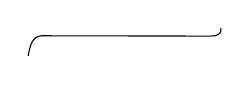
\begin{tikzpicture}[x=.4cm,y=.4cm,baseline=-.2ex]\draw (0,-.45) .. controls (.06,-.08) and (.14,.17) .. (.42,.19)--(5.8,.18) .. controls (6.00,.18) and (6.15,.25) .. (6.12,.43);\end{tikzpicture}}} then the compatibility of $\handwritten{\psi}$ with the unit of $C$ is expressed by the relations
\[
(\mathrm{id}_U\otimes\handwritten{\varepsilon}_U)(\handwritten{\sigma})=(\handwritten{\varepsilon}_U\otimes\mathrm{id}_U)(\handwritten{\sigma})=1,\quad\text{i.e.}\quad\handwritten{\varepsilon\in}1+U^{\handwritten{+}}\overset{\handwritten{\scriptscriptstyle\wedge}}{\otimes}U^{\handwritten{+}}.
\tag*{\handwritten{(2)}}
\]

% source lines 23--26 and bottom handwritten addition
When we have an associativity datum \deleted{on} $\handwritten{\phi}$ for $\unsure{\otimes|\varpi}$, compatible with $F$ and the ordinary associativity of $\otimes$ on $\mathrm{Modf}(k)$, i.e. $A$ is associative, then the compatibility between $\handwritten{\phi}$ and $\handwritten{\psi}$ is expressed by a relation of the sort
\[
\deleted{\handwritten{\sigma}_1\handwritten{\sigma}_2\handwritten{\sigma}_3\handwritten{\sigma}'_1\handwritten{\sigma}'_2\handwritten{\sigma}'_3=1\handwritten{\unsure{\sigma}}}\quad\handwritten{(\mathrm{id}_U\widehat{\otimes}\Delta)(\sigma)\deleted{\sigma^{\unsure{23|13}}\sigma^{12}}=\deleted{1}\sigma^{12}\sigma^{13}}
\tag*{\handwritten{(3)}}
\]
\handwritten{where the \inserted{\unsure{various}\handwritten{\begin{tikzpicture}[x=.4cm,y=.4cm,baseline=-.2ex]\draw (0,-.45) .. controls (.06,-.08) and (.14,.17) .. (.42,.19)--(1.1,.18) .. controls (1.30,.18) and (1.45,.25) .. (1.42,.43);\end{tikzpicture}}} $\sigma^{ij}$ are the 3 images of $\sigma'$ in $U\ominus U\ominus U$ under $x\ominus y\mapsto x\ominus y\ominus1$ and the two other analogous maps.}
